\begin{center}
\large\noindent\fbox{
	\parbox{\textwidth}{
	Utilizzare le function degli Esercizi 4.1 e 4.6 per graficare l'approssimazione della funzione di Runge sull'intervallo \([-6, 6]\), per \(n = 2, 4, 6, \ldots, 40\). Stimare numericamente l'errore commesso in funzione del grado \textit{n} del polinomio interpolante.
	}
}\end{center}

\noindent Il seguente codice Matlab implementa la soluzione al problema dato: 
\lstinputlisting[language=Matlab]{Codici/Cap4/Esercizio7_Cap4.m}
\vspace*{1cm}
\noindent Il grafico seguente mostra i polinomi interpolanti di grado \textit{n}, calcolati utilizzando come punti di interpolazione quelli corrispondenti alle \textit{n} ascisse di Chebyshev. Si ricorda la funzione di Runge scritta come:  \(f(x) = \frac{1}{1+25x^2}\). \\

\hspace{3.5cm}

\begin{figure}[H]
	\centering
    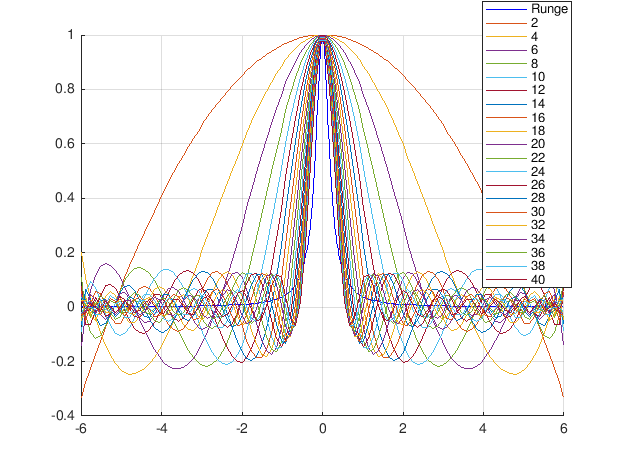
\includegraphics[width=\textwidth,height=\textheight,keepaspectratio]{Codici/Cap4/es7_cap4.png}
\end{figure}

\pagebreak
\noindent Abbiamo quindi calcolato l'errore al variare di $n$ (con $f$ = funzione di Runge e $p_n(x)$ = il suo polinomio interpolante di grado $n$) come segue:

$$
||err|| \approx ||f(x) - p_n(x)||_{\inf}
$$

\noindent Nella seguente tabella si riportano gli errori calcolati: 

\begin{center}
	\begin{tabular}{|c|c|}
		\hline
		$n$ & $\|err\|$ \\
		\hline
		$2$  & $0.9244$ \\
		$4$  & $0.8717$ \\
		$6$  & $0.8217$ \\
		$8$  & $0.7757$ \\
		$10$ & $0.7262$ \\
		$12$ & $0.6866$ \\
		$14$ & $0.6464$ \\
		$16$ & $0.6025$ \\
		$18$ & $0.5568$ \\
		$20$ & $0.5291$ \\
		$22$ & $0.5000$ \\
		$24$ & $0.4696$ \\
		$26$ & $0.4384$ \\
		$28$ & $0.4067$ \\
		$30$ & $0.3747$ \\
		$32$ & $0.3427$ \\
		$34$ & $0.3110$ \\
		$36$ & $0.2855$ \\
		$38$ & $0.2713$ \\
		$40$ & $0.2570$ \\
		\hline
	\end{tabular}
\end{center} 


\noindent Grazie alla scelta delle ascisse di Chebyshev come punti di interpolazione, l'errore diminuisce all'aumentare di \(n\).